
\chapter{Geometría Solar\label{cha:Geometria Solar}}


\section{Geometría del movimiento terrestre}

Como es sabido, el movimiento terrestre se compone de una traslación
alrededor del Sol y un giro sobre su eje\footnote{Las ecuaciones de
  esta sección están implementadas en la función \href{http://search.r-project.org/R/library/solaR/html/fSolD.html}{\texttt{fSolD}} de \texttt{solaR} \cite{Perpinan2012b}}. En el movimiento de traslación
la Tierra se desplaza alrededor del Sol siguiendo una elipse de baja
excentricidad en la que el Sol ocupa uno de los focos. La duración
de este movimiento define un año. Este movimiento está contenido en
el llamado plano de la eclíptica (Figura
\ref{fig:Trayectoria-Sol-Tierra}).


\begin{figure}
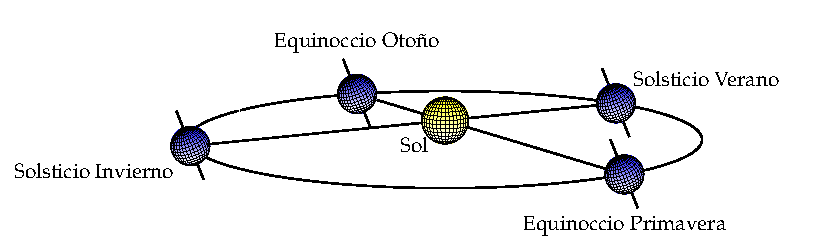
\includegraphics{../figs/PlanoEcliptica}

\caption{Trayectoria Sol-Tierra. Los nombres de los solsticios y equinoccios
están particularizados para el hemisferio Norte.\label{fig:Trayectoria-Sol-Tierra}}

\end{figure}



Debido a la baja excentricidad de la elipse, la distancia entre Sol
y Tierra durante el movimiento de traslación es variable. Una ecuación
simple para describir este distancia está recogida en
\cite{Cooper1969} (ecuación \ref{eq:DistanciaSolTierra_cooper}):

\begin{equation}
r=r_{0}\{1+0.017\sin[\frac{2\pi\cdot(d_{n}-93)}{365}]\}
\label{eq:DistanciaSolTierra_cooper}
\end{equation}
siendo $d_{n}$ el número de día del año (siendo $d_{n}=1$ el 1 de
Enero) y $r_{0}$ es la distancia promedio en este trayecto, denominada
unidad astronómica,
$r_{0}=\SI{1.496e8}{\kilo\metre}=\SI{1}{UA}$\nomenclature[r]{$r$}{Distancia
  entre el Sol y la Tierra}
\nomenclature[r0]{$r_{0}$}{Distancia promedio entre el Sol y la Tierra
  (unidad astronómica)}
\nomenclature[dn]{$d_{n}$}{Día del año}. 

La corrección debida a la excentricidad de la elipse se calcula con
la ecuación \ref{eq:Excentricidad_cooper}:

\begin{equation}
\epsilon_{0}=(\frac{r_{0}}{r})^2=1+0,033\cdot\cos(\frac{2\pi
  d_{n}}{365})
\label{eq:Excentricidad_cooper}
\end{equation}
\nomenclature[e0]{$\epsilon_{0}$}{Corrección debida a la excentricidad
  de la elipse de la trayectoria terrestre alrededor del sol}

En el movimiento de giro la Tierra rota sobre si misma alrededor de
su eje polar, perpendicular al plano ecuatorial terrestre. Entre el
eje polar y el plano de la eclíptica hay un ángulo constante de 23,45\textdegree{}.
Sin embargo, el ángulo entre el plano ecuatorial y la linea que une
Tierra y Sol es variable a lo largo del año. Este ángulo variable
es la causa de las estaciones, de que el Sol aparezca más alto en
los mediodías veraniegos y los días invernales sean más cortos que
los de verano. Utilizando la ecuación \ref{eq:DistanciaSolTierra_cooper}
puede comprobarse sin embargo, que la distancia entre Sol y Tierra
es mayor en el verano que en el invierno del hemisferio Norte. Así,
el efecto debido a la inclinación de los rayos solares es mucho más
apreciable en la meteorología que la distancia entre el Sol y la Tierra. 

Este ángulo se denomina declinación y puede ser calculado de forma
aproximada con la ecuación \ref{eq:Declinacion_cooper} (en grados) y representado en
la figura \ref{fig:Declinacion_cooper} \cite{Cooper1969}. En esta ecuación se supone
que la declinación permanece constante a lo largo de un mismo día.
Asimismo, el criterio de signos supone considerar
positivos los ángulos situados al norte del ecuador terrestre.

\begin{equation}
\delta=\SI{23.45}{\degree}\cdot\sin\left(\frac{2\pi\cdot\left(d_{n}+284\right)}{365}\right)\label{eq:Declinacion_cooper}\end{equation}
\nomenclature[delta]{$\delta$}{Declinación}


\begin{figure}
\begin{centering}
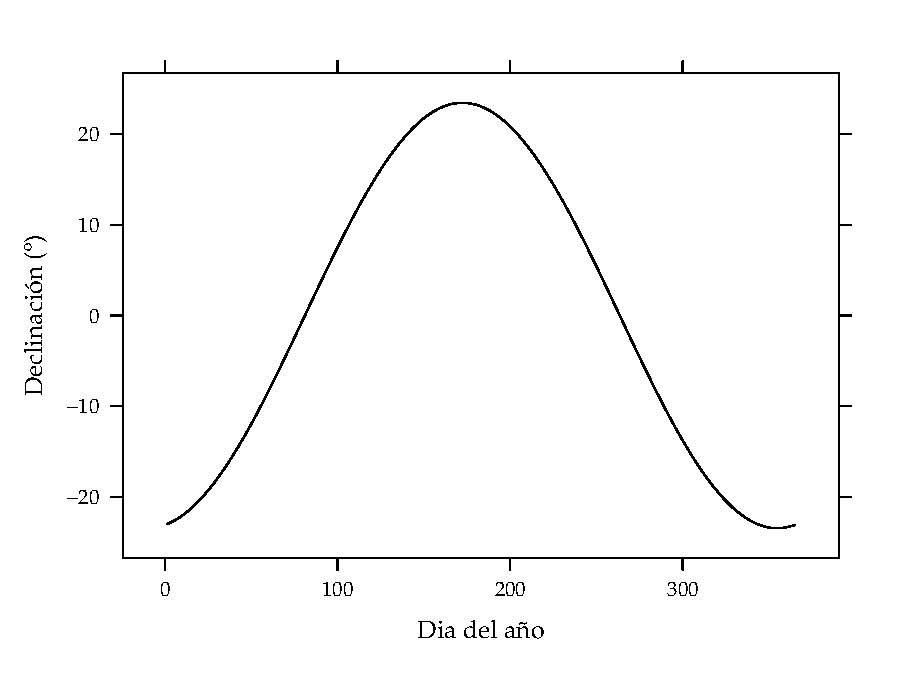
\includegraphics[scale=0.65]{../figs/Declinacion}
\end{centering}

\caption{Declinación.\label{fig:Declinacion_cooper}}

\end{figure}

Otros autores han perfeccionado las ecuaciones anteriores. Son
destacables las aportaciones de Spencer, Michalsky y Strous \cite{Spencer1971, Michalsky1988,
  Strous2011}. Como ejemplo, se detalla a continuación la propuesta de
Spencer (con el resultado en radianes):
\begin{align}
  \label{eq:spencer}
  X &= 2 \pi \cdot (d_n-1)/365\\
  \begin{split}
    \delta &= 0.006918 - 0.399912 \cdot \cos(X) + 0.070257 \cdot \sin(X)\\
    &-  0.006758 \cdot \cos(2 X) + 0.000907 \cdot \sin(2 X)\\
    &- 0.002697 \cdot \cos(3 X) + 0.001480 \cdot \sin(3  X)
  \end{split}\\
  \begin{split}
    \epsilon_{0} &= 1.000110 + 0.034221 \cdot \cos(X) + 0.001280 \cdot
    \sin(X)\\
    &+ 0.000719 \cdot \cos(2 X) + 0.000077 \cdot \sin(2 X)
  \end{split}
\end{align}

El valor de la declinación toma ciertos valores característicos que
definen las estaciones y sus fechas de transición. En los equinoccios%
\footnote{ En el hemisferio Norte el equinoccio de primavera ocurre alrededor
del 21-22 Marzo (día del año 80-81) y el equinoccio de otoño alrededor
del 22-23 Septiembre (día del año 265-266).}% 
la declinación es nula, de forma que el Sol amanece y anochece exactamente
por el Este y Oeste, respectivamente, siendo equivalentes la duración
de día y noche. En el solsticio de junio (21-22 Junio, día del año
172-173) la declinación toma el valor $\delta=23.45\degree$. En el
hemisferio Norte es llamado de verano, produciéndose aquí el día más
largo del año con el Sol amaneciendo por el noreste y anocheciendo
por el noroeste. En el solsticio de Diciembre (21-22 Diciembre, día
del año 355-356) la declinación toma el valor $\delta=-23.45\degree$.
En el hemisferio Norte este solsticio es denominado de invierno, ocurriendo
el día más corto, con el Sol amaneciendo por el sureste y anocheciendo
por el suroeste%
\footnote{Estas consideraciones son traducibles a la óptica del hemisferio Sur
teniendo en cuenta que en este hemisferio el solsticio de junio es
el de invierno, mientras que el de diciembre es el solsticio de verano.%
}. 


\subsection{Movimiento aparente del Sol}

El movimiento combinado que realiza la Tierra es percibido como un
movimiento aparente del Sol a través de la esfera celeste respecto
a la superficie terrestre. Este movimiento aparente puede ser descrito
mediante ecuaciones vectoriales referidas a dos sistemas de referencia,
uno ligado a los ejes terrestres y otro a los ejes locales. Antes,
es necesario situar el punto de observación en la superficie terrestre
mediante su pertenencia a un meridiano y su distancia angular al plano
ecuatorial. 

El meridiano es el arco imaginario que recorre la superficie terrestre
desde el polo Norte hasta el polo Sur, y es el lugar geométrico de
todos los puntos con la misma longitud. La palabra meridiano proviene
del latín \emph{meridies }(mediodía): el mediodía solar es el instante
en el que todos los puntos pertenecientes a un mismo meridiano observan
al Sol en un lugar intermedio entre el amanecer y el ocaso, alcanzando
la altura máxima en el cielo. 

Por otra parte, la intersección de los planos paralelos al ecuatorial
con la superficie terrestre define los circulos de latitud, o lugares
geométricos de aquellos puntos con la misma distancia angular respecto
al ecuador. Dado que el plano ecuatorial define dos hemisferios, la
latitud es un ángulo con signo. De forma equivalente a lo convenido
para la declinación, la latitud tendrá signo positivo para lugares
al norte del Ecuador y negativo para los situados al sur. 

%
\begin{figure}
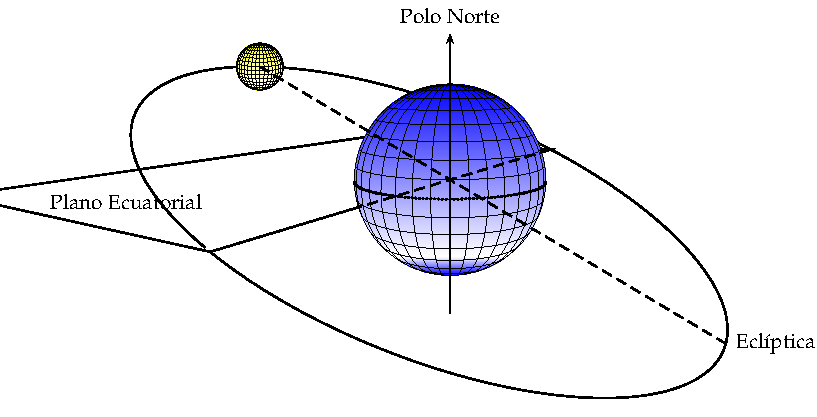
\includegraphics[scale=0.9]{../figs/SoldesdeTierra}

\caption{Sistema geocéntrico según el cual el Sol parece girar alrededor de
la Tierra.\label{fig:ModeloGeocentrico}}

\end{figure}


El sistema basado en los ejes terrestres, ligados a un meridiano,
está compuesto por los tres vectores unitarios siguientes (figuras
\ref{fig:ModeloGeocentrico} y \ref{fig:CoordenadasTerrestres}
): 
\begin{itemize}
\item $\vec{\mu}_{p}$ : vector polar, con la dirección del eje de rotación
terrestre y sentido de sur a norte.
\item $\vec{\mu}_{ec}$: vector ecuatorial, contenido en el plano ecuatorial
terrestre y dirigido hacia la intersección entre este plano y el meridiano
(por tanto, indicando la dirección del mediodía solar).
\item $\vec{\mu}_{\bot}$: vector que resulta del producto vectorial $\vec{\mu}_{p}\times\vec{\mu}_{ec}$,
y por tanto perpendicular al plano definido por los vectores polar
y ecuatorial en dirección hacia el Este.\nomenclature[mup]{$\vec{\mu}_{p}$}{Vector polar}\nomenclature[muec]{$\vec{\mu}_{ec}$}{Vector ecuatorial}\nomenclature[mubot]{$\vec{\mu}_{\bot}$}{Vector perpendicular a los vectores $\vec{\mu}_{c}$ y $\vec{\mu}_{h}$, o a los vectores $\vec{\mu}_{p}$  y $\vec{\mu}_{ec}$}
\end{itemize}
%
\begin{figure}
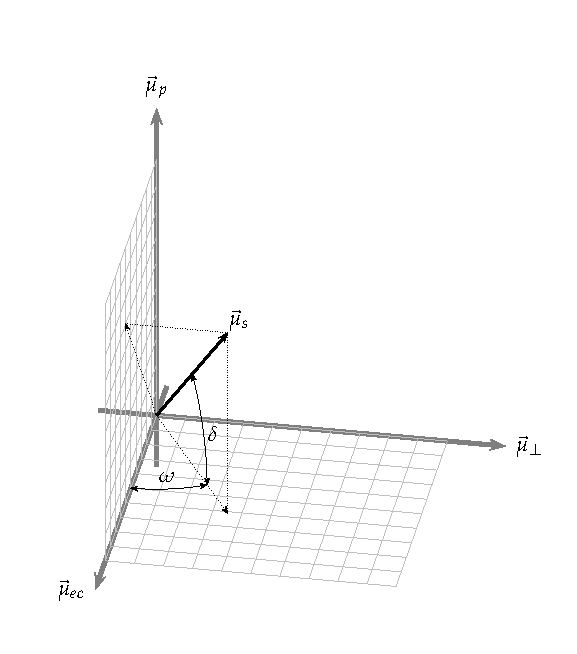
\includegraphics[scale=0.9]{../figs/SistemaCoordenadasTerrestre}

\caption{Sistema de Coordenadas basado en los ejes terrestres.\label{fig:CoordenadasTerrestres}}

\end{figure}


El vector solar, $\vec{\mu}_{s}$, referido a los ejes terrestres
depende de la declinación y de un ángulo denominado hora solar ($\omega$\nomenclature[mus]{$\vec{\mu}_{s}$}{Vector solar}\nomenclature[omega]{$\omega$}{Hora solar o tiempo solar verdadero})
según la ecuación \ref{eq:VectorSolarTerrestre}. El ángulo hora solar,
también denominado tiempo solar verdadero o aparente, mide la diferencia
entre el instante en cuestión y el mediodía solar. De esta forma la
hora solar es nula al mediodía, negativa por la mañana y positiva
por la tarde. Así, cuando el Sol está situado en el primer cuadrante
de este sistema de referencia (figura: \ref{fig:CoordenadasTerrestres})
ya habrá amanecido pero aún no habrá alcanzado el mediodía solar,
y por tanto el ángulo $\omega$ tendrá signo negativo (de ahí el signo
negativo que acompaña a $\vec{\mu}_{\bot}$ en la ecuación \ref{eq:VectorSolarTerrestre})
. Además, en este primer cuadrante el Sol está por encima del plano
ecuatorial y, por tanto, la declinación es positiva.

\begin{equation}
\vec{\mu}_{s}=\left[\cos\left(\delta\right)\cos\left(\omega\right)\right]\cdot\vec{\mu}_{ec}-\left[\cos\left(\delta\right)\sin\left(\omega\right)\right]\cdot\vec{\mu}_{\bot}+\sin\left(\delta\right)\cdot\vec{\mu}_{p}\label{eq:VectorSolarTerrestre}\end{equation}


El sistema basado en los ejes locales está ligado a un meridiano y
a un punto del mismo con latitud $\phi$\nomenclature[phi]{$\phi$}{Latitud}
(figuras \ref{fig:MovimientoAparenteSol} y \ref{fig:CoordenadasLocales}):
\begin{itemize}
\item $\vec{\mu}_{c}$: vector cenital, perpendicular a la superficie terrestre.
\item $\vec{\mu}_{h}:$ vector tangente al meridiano en dirección al ecuador
y, por tanto, dirigido hacia el horizonte sur en el hemisferio norte,
y hacia el horizonte norte en el hemisferio sur.
\item $\vec{\mu}_{\bot}$: vector perpendicular al plano definido por $\vec{\mu}_{c}$
y $\vec{\mu}_{c}$ en dirección hacia el Este   \nomenclature[muc]{$\vec{\mu}_{c}$}{Vector cenital}\nomenclature[muh]{$\vec{\mu}_{h}$}{Vector tangente al meridiano en dirección al ecuador}%
\footnote{Dado que el vector $\vec{\mu}_{h}$ está orientado hacia el ecuador,
para que el vector $\vec{\mu}_{\bot}$ siempre esté dirigido hacia
el Este debe ser el resultado del producto vectorial $\vec{\mu}_{c}\times\vec{\mu}_{h}$
en el hemisferio Norte, y $\vec{\mu}_{h}\times\vec{\mu}_{c}$ en el
hemisferio Sur.%
}.
\end{itemize}
%
\begin{figure}
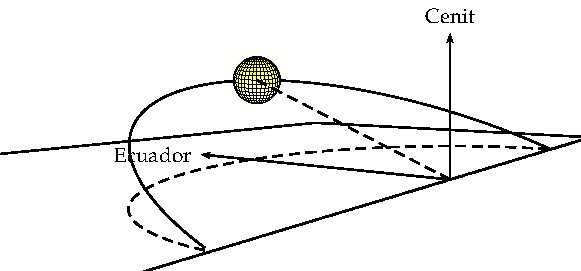
\includegraphics{../figs/SoldesdeTierra2}

\caption{Movimiento aparente del Sol desde un lugar de la Tierra.\label{fig:MovimientoAparenteSol}}

\end{figure}


%
\begin{figure}
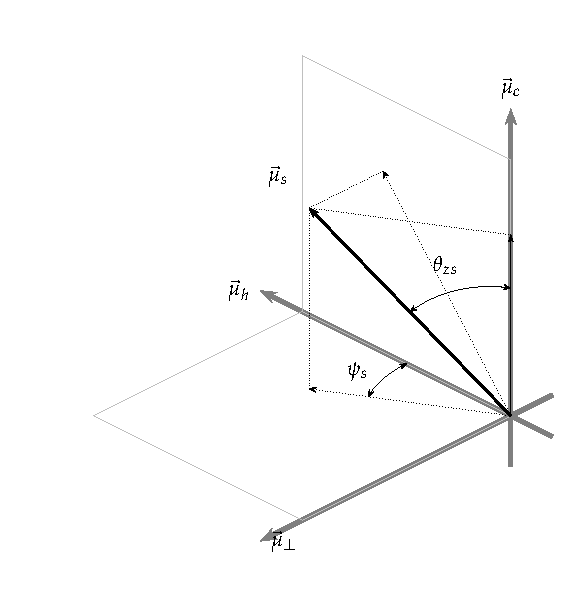
\includegraphics{../figs/SistemaCoordenadasLocal}

\caption{Sistema de Coordenadas basado en los ejes locales.\label{fig:CoordenadasLocales}}

\end{figure}


El vector solar referido a los ejes locales (ecuación \ref{VectorSolarLocales})
depende del ángulo azimutal solar ($\psi_{s}$) y del ángulo cenital
solar ($\theta_{zs}$) (figura \ref{fig:CoordenadasLocales}). El
azimut solar es el ángulo formado por el meridiano solar y el meridiano
del lugar (Sur en el hemisferio Norte y Norte en el hemisferio Sur).
Este ángulo es cero en el mediodía solar, negativo por la mañana y
positivo por la tarde.  \nomenclature[psis]{$\psi_{s}$}{Ángulo acimutal solar}\nomenclature[thetazs]{$\theta_{zs}$}{Ángulo cenital solar}
Este criterio explica el signo negativo que acompaña a $\vec{\mu}_{\bot}$
en la ecuación \ref{VectorSolarLocales}. El ángulo cenital solar
es el ángulo formado por el vector solar y la vertical en el lugar.
Su complementario es la altura o elevación solar.

\begin{equation}
\vec{\mu}_{s}=\left[\cos\left(\psi_{s}\right)\sin\left(\theta_{zs}\right)\right]\cdot\vec{\mu}_{h}-\left[\sin\left(\psi_{s}\right)\sin\left(\theta_{zs}\right)\right]\cdot\vec{\mu}_{\bot}+\cos\left(\theta_{zs}\right)\cdot\vec{\mu}_{c}\label{VectorSolarLocales}\end{equation}


El cambio de unos ejes a otros (figura \ref{fig:RelacionSistemasCoordenadas})
no es más que el resultado de un giro de ángulo igual a la latitud
del lugar, que puede ser expresado mediante una matriz de giro (ecuación
\ref{eq:MatrizGiroCollins})\cite{CollinsII2004}. Sin embargo, en
el ecuador terrestre se produce el cambio de signo de la latitud y
el vector $\vec{\mu}_{h}$ de los ejes locales cambia de sentido respecto
a los ejes terrestres. Estas circunstancias se tienen en cuenta en
la matriz añadiendo el factor $\mathrm{signo}(\phi)$ en la componente
del vector $\vec{\mu}_{h}$ .

%
\begin{figure}
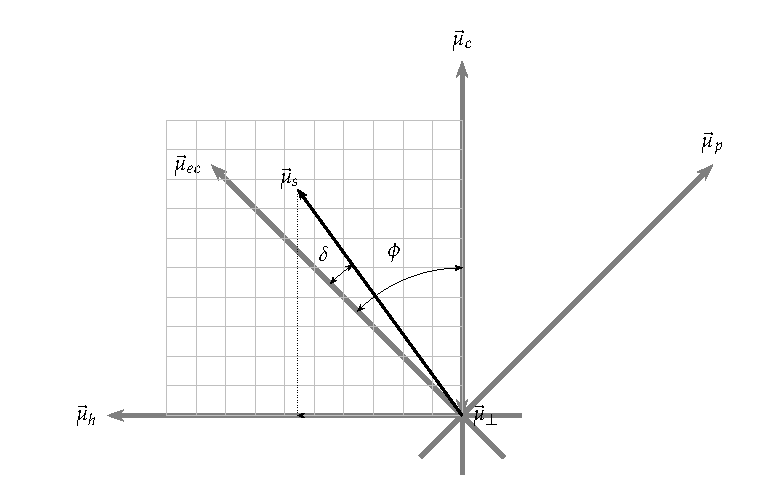
\includegraphics{../figs/RelacionSistemasCoordenadas}

\caption{Relación entre los sistemas de coordenadas terrestre y local (particularizado
para el hemisferio Norte).\label{fig:RelacionSistemasCoordenadas}}

\end{figure}


\begin{equation}
\left(\begin{array}{c}
\vec{\mu}_{ec}\\
\vec{\mu}_{\bot}\\
\vec{\mu}_{p}\end{array}\right)=\left(\begin{array}{ccc}
\mathrm{signo}(\phi)\cdot\sin(\phi) & 0 & \cos(\phi)\\
0 & 1 & 0\\
-\mathrm{signo}(\phi)\cdot\cos(\phi) & 0 & \sin(\phi)\end{array}\right)\left(\begin{array}{c}
\vec{\mu}_{h}\\
\vec{\mu}_{\bot}\\
\vec{\mu}_{c}\end{array}\right)\label{eq:MatrizGiroCollins}\end{equation}


Si se desea hacer la transformación en sentido inverso, basta con
utilizar la traspuesta de esta matriz de giro :

\begin{equation}
\left(\begin{array}{c}
\vec{\mu}_{h}\\
\vec{\mu}_{\bot}\\
\vec{\mu}_{c}\end{array}\right)=\left(\begin{array}{ccc}
\mathrm{signo}(\phi)\cdot\sin(\phi) & 0 & -\mathrm{signo}(\phi)\cdot\cos(\phi)\\
0 & 1 & 0\\
\cos(\phi) & 0 & \sin(\phi)\end{array}\right)\left(\begin{array}{c}
\vec{\mu}_{ec}\\
\vec{\mu}_{\bot}\\
\vec{\mu}_{p}\end{array}\right)\end{equation}


Para deducir las ecuaciones de movimiento solar respecto a generadores
fotovoltaicos, lo más útil es utilizar el vector solar referido a
los ejes locales a partir de la ecuación \eqref{eq:VectorSolarTerrestre}.
Utilizando la matriz de giro correspondiente, el vector solar depende
ahora de la latitud, el ángulo de declinación terrestre y la hora
solar:

\begin{align}
\vec{\mu}_{s} & =\mathrm{signo}(\phi)\cdot\left[\cos\left(\delta\right)\cos\left(\omega\right)\sin\left(\phi\right)-\cos\left(\phi\right)\sin\left(\delta\right)\right]\cdot\vec{\mu}_{h}-\nonumber \\
 & -\left[\cos\left(\delta\right)\sin\left(\omega\right)\right]\cdot\vec{\mu}_{\bot}+\label{eq:VectorSolarLocales2}\\
 & +\left[\cos\left(\delta\right)\cos\left(\omega\right)\cos\left(\phi\right)+\sin\left(\delta\right)\sin\left(\phi\right)\right]\cdot\vec{\mu}_{c}\nonumber \end{align}
y por simple comparación con la ecuación \eqref{VectorSolarLocales}
se deduce la relación entre los ángulos cenital y azimutal con estos
tres ángulos solares\footnote{Ecuaciones implementadas en las
  funciones
  \href{http://search.r-project.org/R/library/solaR/html/fSolI.html}{\texttt{fSolI}}
  y
  \href{http://search.r-project.org/R/library/solaR/html/calcSol.html}{\texttt{calcSol}}
  de \texttt{solaR} \cite{Perpinan2012b}}: 

\begin{equation}
\cos\left(\theta_{zs}\right)=\vec{\mu}_{c}\cdot\vec{\mu}_{s}=\cos\left(\delta\right)\cos\left(\omega\right)\cos\left(\phi\right)+\sin\left(\delta\right)\sin\left(\phi\right)\label{eq:cosThetaZs}\end{equation}


\begin{align}
\vec{\mu_{s}}\cdot\vec{\mu}_{\bot} & =-\sin\left(\psi_{s}\right)\sin\left(\theta_{zs}\right)\\
\vec{\mu_{s}}\cdot\vec{\mu}_{h} & =\mathrm{signo}(\phi)\cdot\cos\left(\psi_{s}\right)\sin\left(\theta_{zs}\right)\\
\cos\left(\psi_{s}\right) & =\mathrm{signo}(\phi)\cdot\frac{\cos\left(\delta\right)\cos\left(\omega\right)\sin\left(\phi\right)-\cos\left(\phi\right)\sin\left(\delta\right)}{\sin\left(\theta_{zs}\right)}\label{eq:cosAzS}\\
\sin(\psi_{s}) &
=\frac{\cos(\delta)\sin(\omega)}{\sin(\theta_{zs})}=\frac{\cos(\delta)\sin(\omega)}{\cos(\gamma_{s})}\label{eq:sinAzS}
\end{align}
donde el ángulo $\gamma_{s}$ es la altura solar, complementario del
ángulo cenital.

Para obtener el valor del ángulo acimutal se debe situar la proyección
del sol en el cuadrante correcto. La función arco coseno permite decidir entre
el primer\footnote{Entre Sur y Oeste} y segundo\footnote{Entre Oeste y
  Norte} cuadrante, o entre tercer\footnote{Entre Norte y Este} y
cuarto\footnote{Entre Sur y Este} cuadrante, pero no es capaz de
discriminar entre el primer y cuarto cuadrante (o entre el segundo y
tercer cuadrante). Esta diferencia se resuelve sabiendo si el sol ha
atravesado ya la línea del mediodía (primer y segundo cuadrante) o aún
no (tercer y cuarto cuadrante). Para resolver este problema la
combinación del arco coseno aplicado a la ecuación (\ref{eq:cosAzS})
junto con el signo de la hora solar es particularmente recomendable.
\nomenclature[gammas]{$\gamma_{s}$}{Altura solar}

En la figura \ref{fig:AlturaRelativaMediodia} se representa la altura
solar al mediodía a lo largo del año en localidades de los dos hemisferios.
Para apreciar la variación de este ángulo con la latitud la altura
está normalizada con el valor máximo anual de este ángulo en cada
localidad. Así, la diferencia entre la altura solar de los meses invernales
y la de los meses veraniegos es más apreciable para las localidades
alejadas del Ecuador.


\begin{figure}
\begin{centering}
\hfill{}\subfloat[Altura mediodía hemisferio Norte.]{\begin{centering}
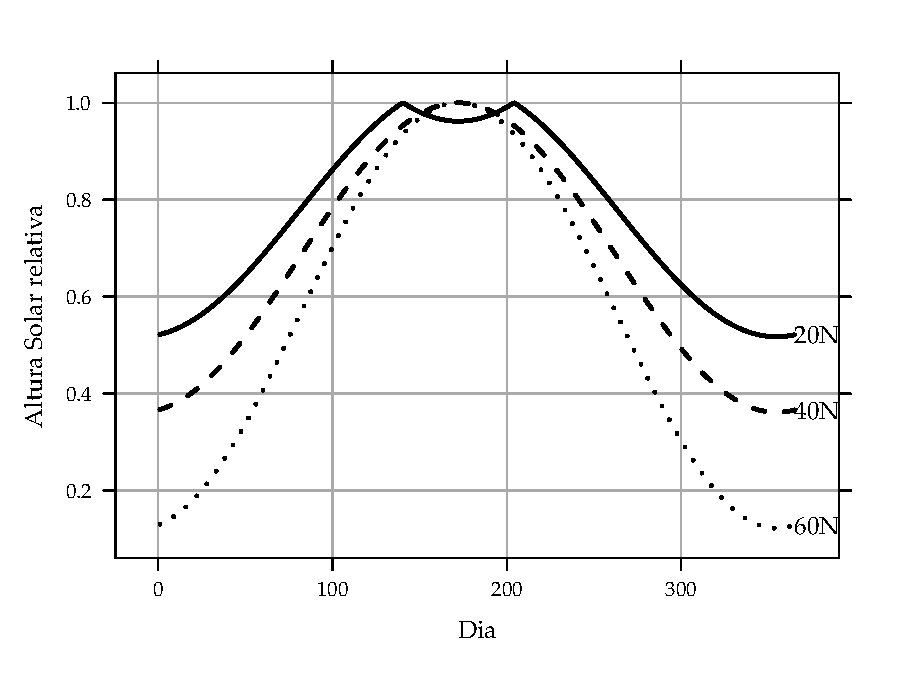
\includegraphics[scale=0.47]{../figs/AlturaSolarMediodiaNORTE}
\par\end{centering}

}\hfill{}\subfloat[Altura mediodía hemisferio Sur.]{\begin{centering}
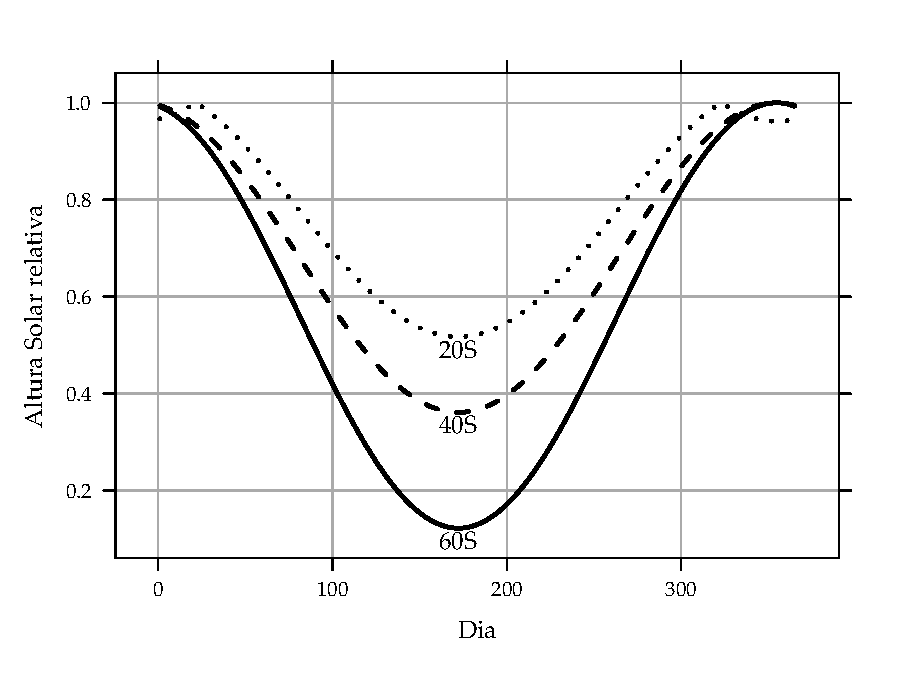
\includegraphics[scale=0.47]{../figs/AlturaSolarMediodiaSUR}
\par\end{centering}

}\hfill{}
\end{centering}

\caption{Altura relativa al mediodía a lo largo del año.\label{fig:AlturaRelativaMediodia}}

\end{figure}

En la figura \ref{fig:DiagramaElevacionAcimutSolar} se muestran dos
diagramas de trayectoria solar definidos por los ángulos de acimut
y elevación para dos latitudes diferentes. Por ejemplo, estos diagramas
muestran que la localidad situada en el hemisferio Sur observa el
Sol con mayor elevación durante el mes de Diciembre. La utilidad de
estos diagramas, además de para comprender el movimiento aparente
del Sol y su relación con la latitud, será mostrada con mayor detalle
al calcular las sombras lejanas que inciden en un sistema fotovoltaico
(sección \ref{sub:Sombras-lejanas}).


\begin{figure}
\begin{centering}
\hfill{}\subfloat[Latitud $60\degree\mathrm{N}$.
]{\begin{centering}
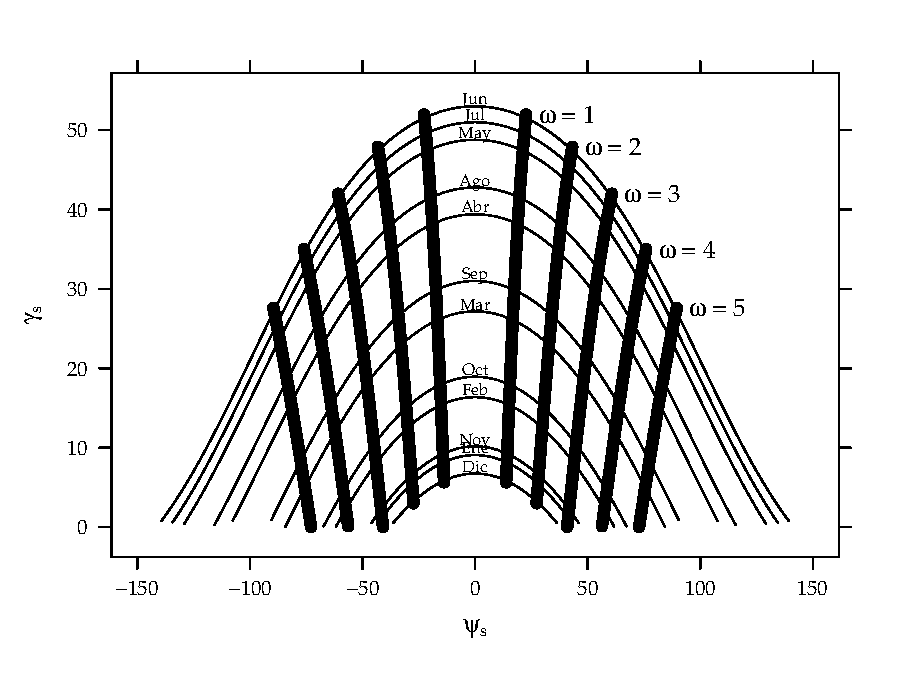
\includegraphics[scale=0.47]{../figs/TrayectoriaSolar60N}
\par\end{centering}

}\hfill{}\subfloat[Latitud $40\degree\mathrm{S}$.
]{\begin{centering}
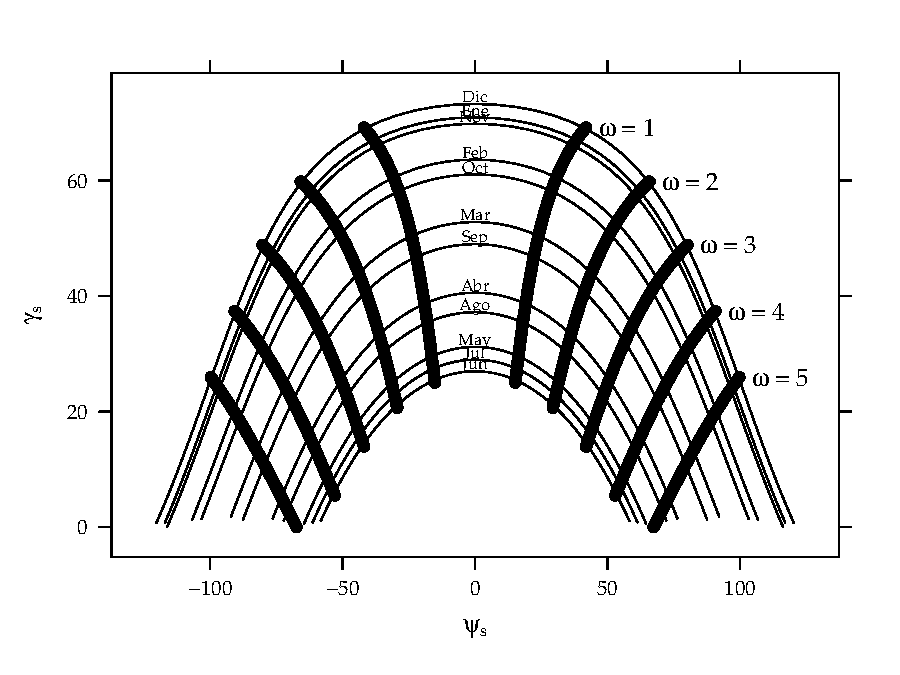
\includegraphics[scale=0.47]{../figs/TrayectoriaSolar40S}
\par\end{centering}

}\hfill{}
\end{centering}

\caption{Diagrama de trayectoria solar según los ángulos de elevación y acimut
en dos localidades terrestres.\label{fig:DiagramaElevacionAcimutSolar}}

\end{figure}

Utilizando la ecuación \ref{eq:cosThetaZs} podemos calcular la hora
solar correspondiente al amanecer y atardecer, situaciones caracterizadas
por una altura solar nula. Por tanto, con $\theta_{zs}=90\degree$,
el ángulo correspondiente al amanecer (negativo según el criterio
de signos) es:

\begin{equation}
\omega_{s}=-\arccos(-\tan\delta\tan\phi)
\label{eq:ws}
\end{equation}
\nomenclature[omegas]{$\omega_{s}$}{Ángulo del amanecer}

La duración de un día \footnote{Para traducir un valor angular en
  grados a un número de horas es suficiente tener en cuenta que un día
  completo, correspondiente a $360\degree$, tiene una duración
  media de 24 horas. Por tanto, $\SI{1}{\hour}$ equivale a
  $15\degree$.}  cualquiera es $2\cdot|\omega_{s}|$,
dependiente del día del año a través de la declinación y del lugar de
la superficie terrestre a través de la latitud. La figura
\ref{fig:Duracion-del-Dia} permite observar que la duración del día es
constante en los lugares ecuatoriales y que la diferencia de esta
duración en los equinoccios y solsticios es tanto más apreciable
cuanto mayor sea la latitud.


\begin{figure}
\begin{centering}
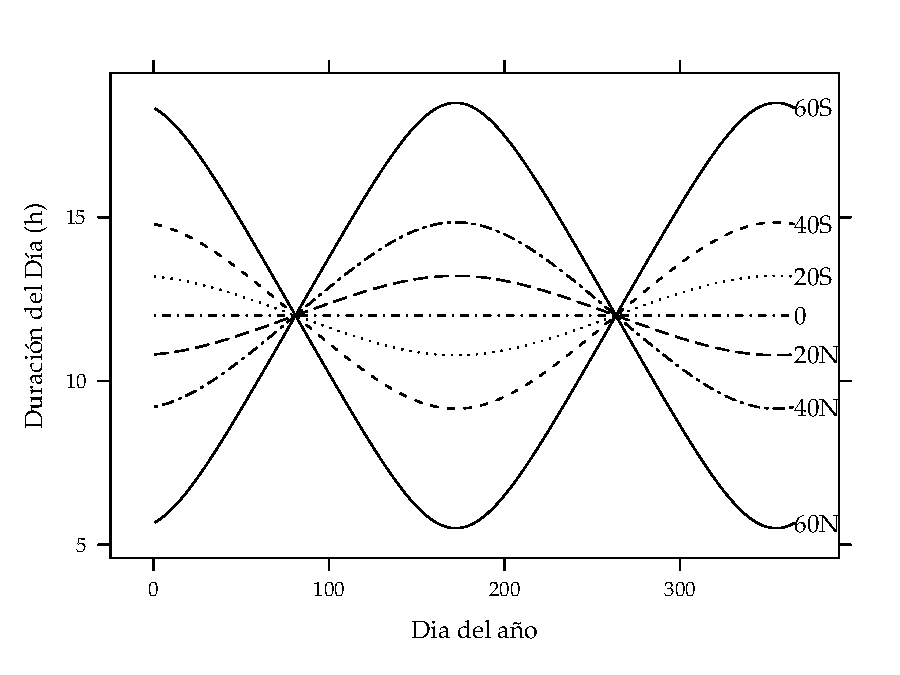
\includegraphics[scale=0.65]{../figs/DuracionDia}
\end{centering}

\caption{Duración del día en diferentes latitudes.\label{fig:Duracion-del-Dia}}

\end{figure}

Desde los círculos polares ($\phi=\pm 66.55 \degree$) hasta los polos,
en algunos días del año el sol permanece siempre por encima del
horizonte. A estos días de veinticuatro horas de duración se les
denomina días polares. En su contrapartida, las noches de veinticuatro
horas, el sol permanece continuamente por debajo del horizonte. En
estos días, el valor de $-\tan\delta\tan\phi$ es menor que -1 (días
polares) o mayor que 1 (noches polares), luego la ecuación
(\ref{eq:ws}) debe ampliarse para tenerlo en cuenta ($\omega_s$ expresado en radianes):

\begin{equation}
\omega_s=\begin{cases}
-\arccos(-\tan\delta\tan\phi)& \text{si $|\tan\delta\tan\phi|<1$}\\
  -\pi& \text{si $-\tan\delta\tan\phi<-1$}\\
  0& \text{si $-\tan\delta\tan\phi>1$}
\end{cases}
\label{ws_polar}
\end{equation}


\subsection{Hora oficial y hora solar}

Para calcular el tiempo solar aparente a partir de la hora oficial
(la que podemos leer en un reloj convencional), es necesario realizar
varias correcciones. Entendamos primero el origen de la hora oficial
y a continuación analicemos brevemente las complicaciones derivadas
de emplear el movimiento terrestre como medida temporal.

La hora oficial en un punto del planeta es una medida del tiempo ligada
a un meridiano, denominado huso horario, que sirve de referencia para
una zona determinada. En la actualidad existen 39 zonas temporales
diferentes, si bien la primera propuesta realizada en 1879 dividía
al planeta en 24 zonas que abarcaban $15\degree$ cada una. Todos
los husos horarios se cuentan a partir del meridiano de Greenwich
(denominado huso horario GMT) considerando positivos aquellos situados
al Este de este huso horario origen. Por ejemplo, a pesar de que la
península ibérica se encuentra en la región geográfica de influencia
del meridiano de Greenwich, razones de índole práctica ocasionan que
la hora oficial de la España peninsular se rija por el huso horario
de Centroeuropa%
\footnote{El lector interesado puede encontrar más información sobre los husos
horarios en \url{http://en.wikipedia.org/wiki/Time_zone}%
}. Este huso horario está situado en $15\degree\mathrm{E}$ y de ahí
que se le denomine como GMT+1 . De esta forma, la hora oficial en
la España peninsular adelanta en promedio 60 minutos a la hora que
corresponde al meridiano de Greenwich. Así se entiende la necesidad
de añadir una corrección que tenga en cuenta la distancia angular
entre el meridiano local y la longitud del huso horario. Calculamos
esta corrección con $\Delta\lambda=\lambda_{L}-\lambda_{H}$, siendo
$\lambda_{L}$ la longitud local \nomenclature[lambdaL]{$\lambda_{L}$}{Longitud de la localidad}y
$\lambda_{H}$ la longitud del huso horario\nomenclature[lambdaH]{$\lambda_{H}$}{Longitud del huso horario}.
Con el criterio de signos que considera positivas las longitudes de
los meridianos situados al este del meridiano de Greenwich, $\Delta\lambda$
\nomenclature[deltaL]{$\Delta \lambda$}{Diferencia entre la longitud local y la longitud del huso horario}es
positiva cuando la localidad está situada al este de su huso horario.
En este caso, su hora oficial estará retrasada respecto a su hora
solar local. Como diferencia adicional entre la hora oficial y la
hora solar local, debe tenerse en cuenta que algunos estados deciden
utilizar un horario de verano por motivos de ahorro energético adelantando
en 60 minutos la hora oficial. 

Ahora bien, el empleo del movimiento de traslación y rotación terrestre
como una medida de tiempo constante no está exento de problemas. Es
posible comprobar que la duración del día solar real, definido como
el tiempo que transcurre entre dos pasos consecutivos del Sol por
el meridiano local, varía a lo largo del año. El promedio anual de
esta variación es nulo, y de ahí que se emplee el denominado día solar
medio cuya duración es constante a lo largo del año e igual al valor
medio de la duración del día solar real. El día solar medio ha estado
tradicionalmente ligado a la denominación GMT (\emph{Greenwich Mean
Time}), aunque desde 1972 la medida del día solar medio ha sido sustituida
por la UTC (\emph{Coordinated Universal Time}). La relación entre
el tiempo solar medio y el tiempo solar real o aparente se expresa
en la denominada ecuación del tiempo, $\mathrm{EoT}$\nomenclature[EoT]{EoT}{Ecuación del tiempo}.
Esta ecuación incluye dos de las causas más importantes por las que
la duración del día varía con el paso de las estaciones: la orbita
elíptica alrededor del Sol y el ángulo de inclinación del plano de
la eclíptica respecto al plano ecuatorial. La ecuación \ref{eq:EoT}
(figura \ref{fig:EoT}) proporciona el valor de la ecuación del tiempo
en minutos \cite{Whitman2003}.

\begin{equation}
\mathrm{EoT}=229.18\cdot\left(-0.0334\cdot\sin(M)+0.04184\cdot\sin\left(2\cdot
    M+3.5884\right)\right)\label{eq:EoT}\end{equation}
donde $M$ (en radianes) está relacionado con el día del año a través de la relación
$M=\frac{2\cdot\pi}{365.24}\cdot d_{n}$.

%
\begin{figure}


\begin{centering}
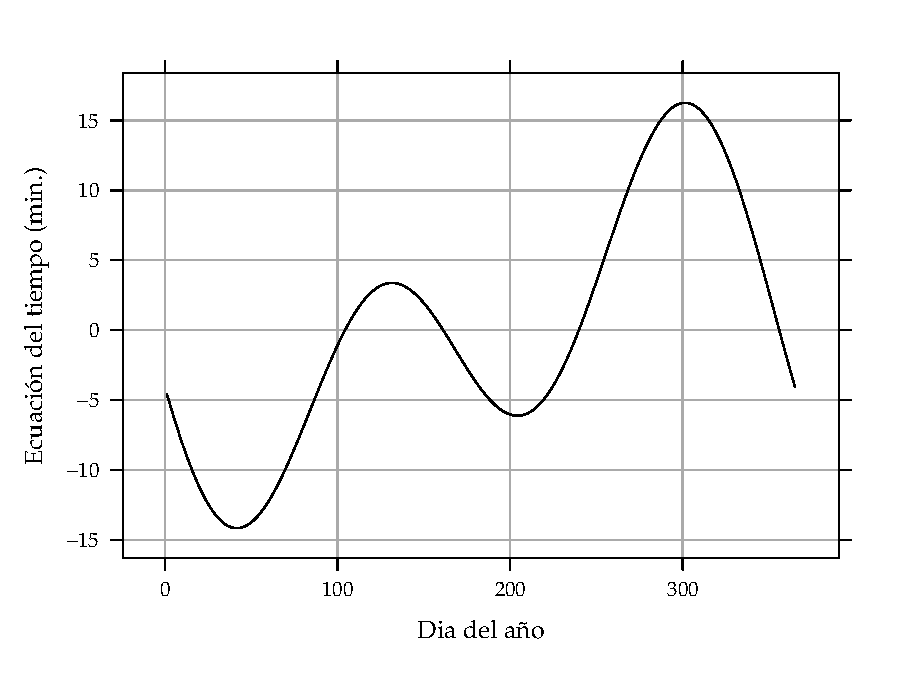
\includegraphics[scale=0.65]{../figs/EoT}
\end{centering}

\caption{Ecuación del tiempo (minutos)\label{fig:EoT}}



\end{figure}


Las correcciones necesarias\footnote{Implementadas en la función
  \href{http://search.r-project.org/R/library/solaR/html/local2Solar.html}{\texttt{local2Solar}} de \texttt{solaR} \cite{Perpinan2012b}} para traducir la hora oficial, $\mathrm{TO}$,
en la hora solar real, $\omega$, quedan sintetizadas en la ecuación
\ref{eq:HoraSolar}:\nomenclature[TO]{TO}{Hora oficial}\begin{equation}
\omega=15\cdot(\mathrm{TO}-\mathrm{AO}-12)+\Delta\lambda+\frac{\mathrm{EoT}}{4}\label{eq:HoraSolar}\end{equation}
donde $\mathrm{AO}$ es el adelanto oficial durante el horario de
verano\nomenclature[AO]{AO}{Adelanto oficial durante el horario de verano}.
En esta ecuación, $\mathrm{TO}$ y $\mathrm{AO}$ están en horas,
$\omega$, $\Delta\lambda$ están en grados, y $\mathrm{EoT}$ está
en minutos.

Por ejemplo, calculemos la hora solar real correspondiente al día
23 de Abril de 2010 a las 12 de la mañana, hora oficial de la ciudad
de A Coruña, Galicia. Esta localidad está contenida en el meridiano
de longitud $8.38\degree\mathrm{W}$ y su hora oficial está regida
por el huso horario GMT+1. Por tanto $\lambda_{L}=-8.38\degree$,
$\lambda_{H}=15\degree$ y $\Delta\lambda=-23.38\degree$. En España
se aplica el horario de verano y este día está incluido en el período
afectado, $\mathrm{AO}=1$. Por último, para este día $\mathrm{EoT=\SI{1.78}{\minute}}$.
Con todos estos cálculos parciales obtenemos $\omega=-37.94\degree$
(aproximadamente las 9 y media de la mañana, hora solar real). El
Sol culminará ($\omega=0$) cuando sean las 14:31, hora oficial.


\section{Geometría de la radiación incidente en sistemas fotovoltaicos}
\label{sec:geometria-sistemas}

Es conocimiento común que la potencia entregada por un generador
fotovoltaico es tanto mayor cuanto mayor sea el nivel de radiación
efectiva incidente en el mismo. El cálculo de la radiación efectiva
incluye las pérdidas por reflexión, efecto relacionado con el ángulo
formado entre la línea que une el generador con el sol y la
perpendicular al plano del módulo.  Cuanto mayor es este ángulo, mayor
es la radiación reflejada, efecto que podemos experimentar si
observamos desde diferentes ángulos la intensidad de nuestra imagen en
una superficie acristalada de un edificio.

Teniendo en cuenta que la radiación directa es, en general,
proporcionalmente superior a la radiación difusa, y que las pérdidas
por reflexión disminuyen si el apuntamiento al sol mejora, se diseñan
los sistemas de seguimiento solar. Su objetivo común es reducir el
ángulo formado entre el vector solar y el vector director del plano
generador a lo largo del movimiento celeste del sol. Las diferentes
técnicas de seguimiento buscan concretar este objetivo general
sacrificando un apuntamiento perfecto en aras de conseguir sistemas
estructurales más económicos y mejores aprovechamientos del terreno.

A continuación se desarrollan un conjunto de
ecuaciones\footnote{Implementadas en la función
  \href{http://search.r-project.org/R/library/solaR/html/fTheta.html}{\texttt{fTheta}}
  de \texttt{solaR} \cite{Perpinan2012b}} para modelar el
comportamiento de las diferentes técnicas de seguimiento. Este primer
paso servirá para generar estimaciones de energía producida por cada
uno de ellos, estimaciones que serán recogidas en gráficas
comparativas de radiación incidente (sección
\ref{sec:comparacion-sistemas}).  También emplearemos estas ecuaciones
para estudiar el impacto de las sombras mutuas entre seguidores
(apartado \ref{sub:Sombras-mutuas}).

El mejor método de seguimiento desde la perspectiva de la radiación
efectiva incidente o de la producción eléctrica es el de doble eje,
que consigue apuntar al sol con precisión a lo largo de todo su
recorrido. En los sistemas de concentración es imprescindible adoptar
este método, ya que los concentradores, grosso modo, son ciegos a la
radiación difusa y tan sólo son capaces de aprovechar el componente
directo de la radiación.

En el siguiente puesto de los que optimizan la producción se encuentra
el seguimiento acimutal, que sacrifica un movimiento (inclinación del
generador) para conseguir sistemas más económicos. El método consiste
en girar de este a oeste sobre un eje vertical. 

Otro planteamiento diferente es el utilizado por el seguimiento
polar. El único eje sobre el que se produce el giro está inclinado de
forma paralela al eje de rotación de la Tierra, consiguiendo que el
generador aparezca al sol como perpendicular a sus rayos durante gran
parte del recorrido. No obstante, las complicaciones estructurales y
de giro, y la dificultad de su implantación en grandes plantas han
provocado que su uso sea ocasional.

Por último se debe mencionar el método de seguimiento horizontal con
eje Norte-Sur. Sus ventajas son la sencillez y estabilidad estructural
(el eje es horizontal y paralelo al terreno, con tantos puntos de
apoyo como se consideren necesarios), la facilidad de motorización,
así como el mejor aprovechamiento del terreno en relación a un sistema
de doble eje.


\subsection{Sistema estático}

Los sistemas más comunes basan su funcionamiento en generadores
fotovoltaicos orientados hacia el Ecuador Terrestre (Sur en el
hemisferio Norte, Norte en el hemisferio Sur) con una inclinación que
depende de la latitud. En este caso, el vector director del plano del
generador, referido a los ejes locales es:

\begin{equation}
\vec{\mu}_{\beta}=\sin(\beta)\cdot\vec{\mu}_{h}+\cos(\beta)\cdot\vec{\mu}_{c}\end{equation}
\nomenclature[mubeta]{$\vec{\mu}_{\beta}$}{Vector director del plano de un generador estático}y
el ángulo entre este vector director y el vector solar es:

\begin{align}
\cos(\theta_{s}) & =\vec{\mu}_{\beta}\cdot\vec{\mu}_{s}\nonumber \\
 & =\mathrm{signo}(\phi)\cdot\bigl[\sin(\beta)\cos\left(\delta\right)\cos\left(\omega\right)\sin\left(\phi\right)-\nonumber \\
 & -\sin(\beta)\cos\left(\phi\right)\sin\left(\delta\right)\bigr]+\nonumber \\
 & +\cos(\beta)\cos\left(\delta\right)\cos\left(\omega\right)\cos\left(\phi\right)+\nonumber \\
 & +\cos(\beta)\sin\left(\delta\right)\sin\left(\phi\right)=\nonumber \\
 & =\cos\left(\delta\right)\cos\left(\omega\right)\cos\left(\beta-|\phi|\right)-\mathrm{signo}(\phi)\cdot\sin(\delta)\sin\left(\beta-|\phi|\right)\label{eq:cosThetaEstaticaSUR}\end{align}
\nomenclature[thetas]{$\theta_{s}$}{Ángulo de incidencia o ángulo entre el vector solar y el vector director de una superficie}

%
\begin{figure}
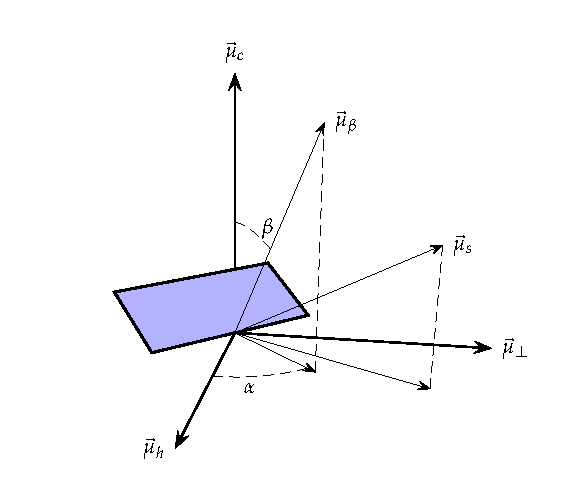
\includegraphics{../figs/AngulosSistemaEstatico}

\caption{Ángulos y vectores en un sistema estático.\label{fig:Estatica}}

\end{figure}


No siempre es posible dotar al generador de la orientación hacia el
ecuador terrestre. En estos casos, el vector director es (figura \ref{fig:Estatica}):

\begin{equation}
\vec{\mu}_{\beta}=[\sin(\beta)\cos(\alpha)]\cdot\vec{\mu}_{h}-[\sin(\beta)\sin(\alpha)]\cdot\vec{\mu}_{\bot}+\cos(\beta)\cdot\vec{\mu}_{c}\end{equation}
y el coseno del ángulo con el vector solar (también denominado ángulo
de incidencia):

\begin{align}
\cos(\theta_{s}) & =\mathrm{signo}(\phi)\cdot\bigl[\sin(\beta)\cos(\alpha)\cos\left(\delta\right)\cos\left(\omega\right)\sin\left(\phi\right)-\nonumber \\
 & -\sin(\beta)\cos(\alpha)\cos\left(\phi\right)\sin\left(\delta\right)\bigr]+\nonumber \\
 & +\sin(\beta)\sin(\alpha)\cos\left(\delta\right)\sin\left(\omega\right)+\nonumber \\
 & +\cos(\beta)\cos\left(\delta\right)\cos\left(\omega\right)\cos\left(\phi\right)+\nonumber \\
 & +\cos(\beta)\sin\left(\delta\right)\sin\left(\phi\right)\label{eq:cosThetaEstatica}\end{align}


La evolución del coseno del ángulo de incidencia a lo largo del día
y año para un sitio con latitud $40\degree\mathrm{N}$ se representa
en la figura \ref{fig:cosThetaEst}. Es evidente que el ángulo de
incidencia es más favorable en las horas cercanas al mediodía solar.

%
\begin{figure}
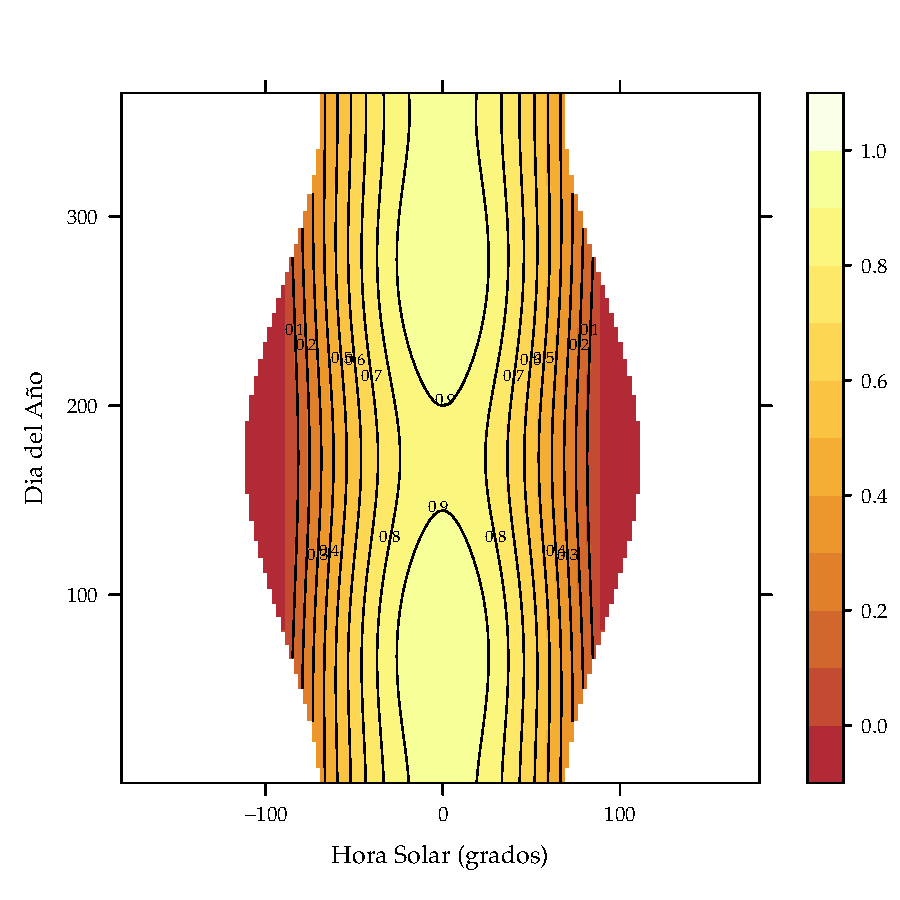
\includegraphics[scale=0.75]{../figs/cosThetaEst_40N}

\caption{Coseno del ángulo de incidencia en un sistema estático a lo largo
del día y año para un sitio con latitud $40\degree\mathrm{N}$.\label{fig:cosThetaEst}}

\end{figure}



\subsection{Eje horizontal Norte-Sur}

Cuando el movimiento se realiza sobre un eje orientado en sentido
norte-sur, considerando que el plano del generador es siempre paralelo
a este eje, el vector director del plano del generador es (figura
\ref{fig:HorizontalNS}):

\begin{equation}
\vec{\mu}_{ns}=-\sin(\psi_{ns})\cdot\vec{\mu}_{\bot}+\cos(\psi_{ns})\cdot\vec{\mu}_{c}\end{equation}
\nomenclature[muns]{$\vec{\mu}_{ns}$}{Vector director de la superficie de un seguidor de eje horizontal Norte-Sur}donde
\begin{equation}
\begin{array}{ccc}
\psi_{ns}<0 & \mathrm{cuando} & \omega<0\end{array}\end{equation}


%
\begin{figure}
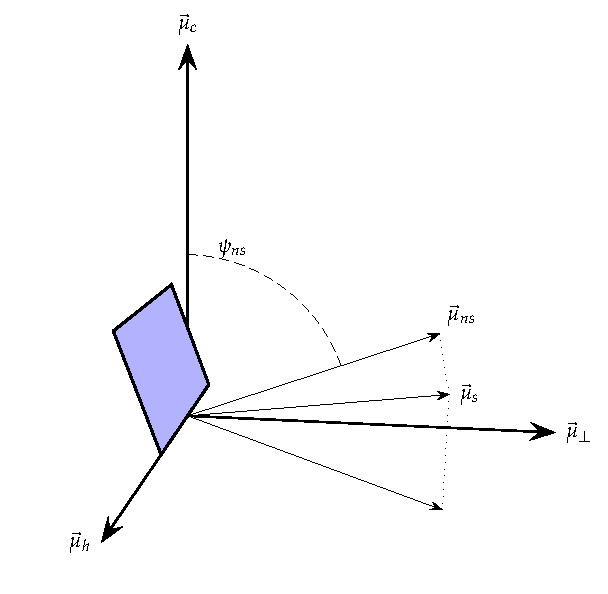
\includegraphics[scale=0.85]{../figs/AngulosSistemaHorizontalNS}

\caption{Vectores y ángulos en un SFCR de eje horizontal Norte-Sur.\label{fig:HorizontalNS}}

\end{figure}


La condición de buen apuntamiento en esta tipología implica que el
vector $\vec{\mu}_{ns}$ es paralelo a la proyección del vector solar
contenida en el plano definido por los vectores $\vec{\mu}_{\bot}$
y $\vec{\mu}_{c}$:

\begin{equation}
\frac{\sin(\psi_{ns})}{\cos\left(\delta\right)\sin\left(\omega\right)}=\frac{\cos(\psi_{ns})}{\cos\left(\delta\right)\cos\left(\omega\right)\cos\left(\phi\right)+\sin\left(\delta\right)\sin\left(\phi\right)}\end{equation}
y por tanto:

\begin{align}
\tan(\psi_{ns}) & =\frac{\cos(\delta)\sin(\omega)}{\cos\left(\delta\right)\cos\left(\omega\right)\cos\left(\phi\right)+\sin\left(\delta\right)\sin\left(\phi\right)}=\nonumber \\
 & =\frac{\cos(\delta)\sin(\omega)}{\cos(\theta_{z})}=\nonumber \\
 & =\frac{\sin(\omega)}{\cos(\omega)\cos(\phi)+\tan(\delta)\sin(\phi)}\label{eq:tanPsi_NS1}\end{align}


Utilizando la ecuación \eqref{eq:sinAzS}, esta ecuación puede escribirse
de forma alternativa como:

\begin{equation}
\tan(\psi_{ns})=\frac{\sin(\psi_{s})}{\tan(\gamma_{s})}\label{eq:tanPsiNS2}\end{equation}


De esta manera, el ángulo con el vector solar es:

\begin{align}
\cos(\theta_{s}) & =\vec{\mu}_{ns}\cdot\vec{\mu}_{s}=\nonumber \\
 & =\sin(\psi_{ns})\cos\left(\delta\right)\sin\left(\omega\right)+\cos(\psi_{ns})\left(\cos(\delta)\cos(\omega)\cos(\phi)+\sin(\delta)\sin(\phi)\right)=\nonumber \\
 & =\cos(\delta)\left[\sin(\psi_{ns})\sin(\omega)+\cos(\psi_{ns})\left(\cos(\omega)\cos(\phi)+\tan(\delta)\sin(\phi)\right)\right]\label{eq:cosThetaNS1}\end{align}


Para eliminar el ángulo $\psi_{ns}$ se tiene en cuenta que el factor
que multiplica a $\cos(\delta)$ es de la forma $A\cdot\sin(\psi_{ns})+B\cdot\cos(\psi_{ns})$,
y además $\tan(\psi_{ns})=A/B$. Haciendo una transformación con esta
observación, se obtiene:

\begin{align}
A\cdot\sin(\psi_{ns})+B\cdot\cos(\psi_{ns}) & =B\cdot\frac{\sin^{2}(\psi_{ns})}{\cos(\psi_{ns})}+B\cdot\cos(\psi_{ns})\nonumber \\
 & =\frac{B}{\cos(\psi_{ns})}
\label{eq:factorNS}\end{align}
y además

\begin{equation}
\cos(\psi_{ns}) =\sqrt{\frac{1}{1+\tan^{2}(\psi_{ns})}} =
\frac{B}{\sqrt{A^{2}+B^{2}}}
\label{cosBetaHorizontal}
\end{equation}


Por tanto, combinando las ecuaciones \eqref{eq:factorNS} y
\eqref{cosBetaHorizontal} obtenemos: 
\begin{equation}
A\cdot\sin(\psi_{ns})+B\cdot\cos(\psi_{ns})=\sqrt{A^{2}+B^{2}}\label{reagrupa_tan}\end{equation}

De esta forma, en la ecuación \eqref{eq:cosThetaNS1} el factor
mencionado puede reagruparse para escribir el coseno del ángulo de
incidencia:

\begin{equation}
\cos(\theta_{s})=\cos(\delta)\sqrt{\sin^{2}(\omega)+\left(\cos(\omega)\cos(\phi)+\tan(\delta)\sin(\phi)\right)^{2}}\label{eq:cosThetaNS_Final}\end{equation}


Es evidente que el ángulo de inclinación del generador respecto a
la superficie horizontal es:

\begin{equation}
\beta=\left|\psi_{ns}\right|\label{eq:BetaNS}\end{equation}
y la orientación del seguidor es constante en valor con signo cambiante
según la posición solar respecto al mediodía:\begin{equation}
\alpha=\frac{\pi}{2}\cdot\mathrm{signo}(\omega)\end{equation}
\nomenclature[psins]{$\psi_{ns}$}{Ángulo de inclinación (con signo) de un seguidor de eje horizontal Norte-Sur}

La evolución del coseno del ángulo de incidencia a lo largo del día
y año para un sitio con latitud $40\degree\mathrm{N}$ se representa
en la figura \ref{fig:cosThetaHoriz}. Es evidente que el movimiento
realizado por este seguidor mejora sustancialmente el ángulo de incidencia
respecto a un sistema estático (\ref{fig:cosThetaEst}).

%
\begin{figure}
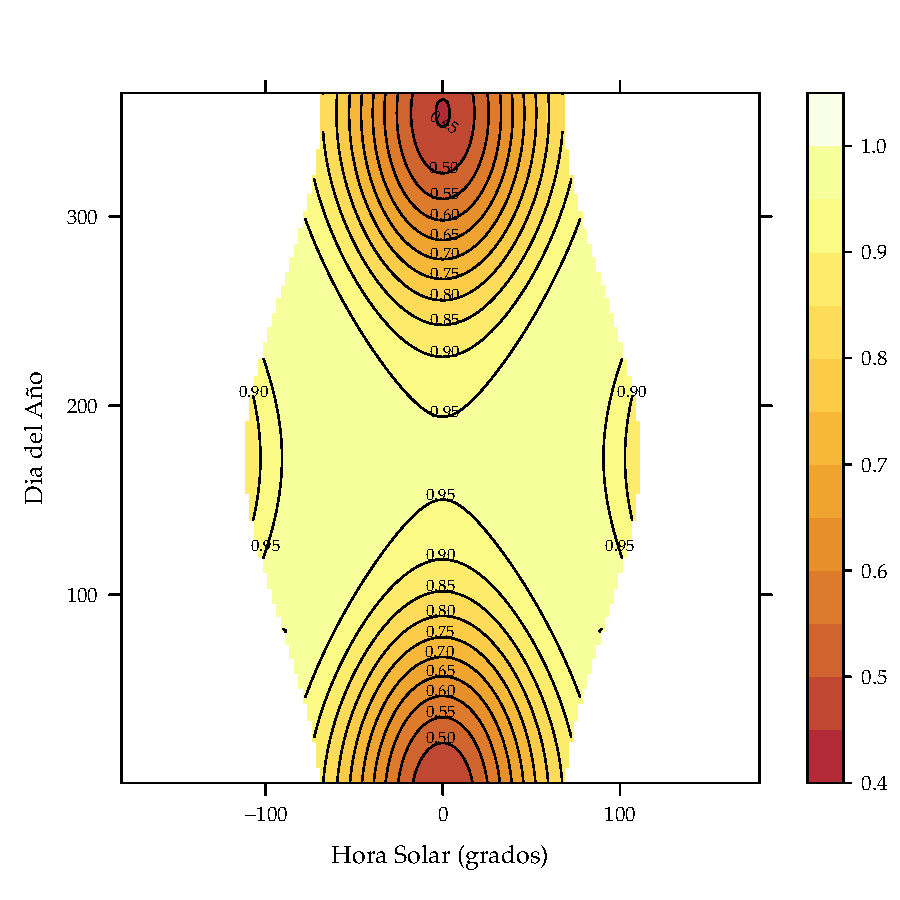
\includegraphics[scale=0.75]{../figs/cosThetaHoriz_40N}

\caption{Coseno del ángulo de incidencia en un sistema de eje horizontal Norte-Sur
a lo largo del día y año para un sitio con latitud $40\degree\mathrm{N}$.\label{fig:cosThetaHoriz}}

\end{figure}


Cabe la posibilidad de inclinar el plano generador respecto al eje
de giro para mejorar el ángulo de incidencia (figura \ref{fig:SeguidoresNSInclinado}),
y por tanto la producción resultante. Para el desarrollo de las ecuaciones,
se emplearán como ejes de referencia unos ejes móviles ligados al
propio seguidor:
\begin{itemize}
\item $\vec{\mu}_{eje}$\nomenclature[mueje]{$\vec{\mu}_{eje}$}{Vector del eje de un seguidor de eje horizontal Norte-Sur}
: coincidente con el eje del seguidor, y también con el vector $\vec{\mu_{h}}$
(figura \ref{fig:CoordenadasLocales}).
\item $\vec{\mu}_{D}$\nomenclature[muD]{$\vec{\mu}_{D}$}{Vector perpendicular al eje de giro de un seguidor de eje horizontal Norte-Sur y contenido en el plano perpendicular al plano del generador}:
vector perpendicular al eje de giro y contenido en el plano perpendicular
al plano del generador.
\item $\vec{\mu}_{\bot}$: vector perpendicular al plano definido por los
dos vectores anteriores.
\end{itemize}
Es inmediato comprobar que el vector director es, en este sistema
de referencia, equivalente al de un sistema estático:

%
\begin{figure}
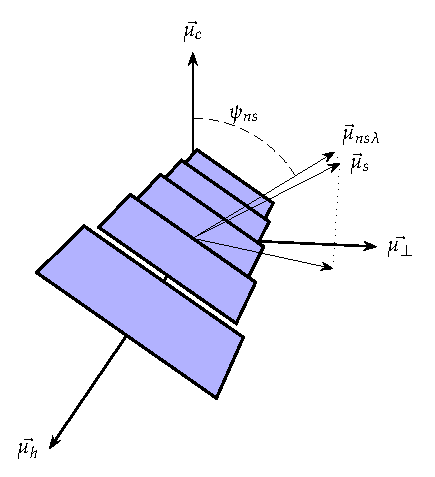
\includegraphics{../figs/AngulosSistemaHorizontalNSLamasInclinadas}

\caption{Lamas inclinadas en seguidor de eje horizontal Norte-Sur.\label{fig:SeguidoresNSInclinado}}

\end{figure}


\begin{equation}
\left.\vec{\mu}_{ns\lambda}\right|_{ejes\ moviles}=\vec{\mu}_{\beta}\end{equation}


\begin{equation}
\left.\vec{\mu}_{ns\lambda}\right|_{ejes\ moviles}=\sin(\lambda)\cdot\vec{\mu}_{eje}+\cos(\lambda)\vec{\mu}_{D}\end{equation}
donde se ha utilizado el ángulo $\lambda$ para referirnos a la inclinación
del plano generador respecto al eje de giro.  \nomenclature[lambda]{$\lambda$}{Inclinación de un generador respecto al eje de giro de un seguidor de eje horizontal Norte-Sur}
La relación entre este sistema de referencia y el sistema local utilizado
hasta ahora viene definido por otra matriz de giro:

\begin{equation}
\left[\begin{array}{c}
\vec{\mu}_{eje}\\
\vec{\mu}_{H}\\
\vec{\mu}_{D}\end{array}\right]=\left[\begin{array}{ccc}
1 & 0 & 0\\
0 & \cos(\psi_{ns}) & \sin(\psi_{ns})\\
0 & -\sin(\psi_{ns}) & \cos(\psi_{ns})\end{array}\right]\cdot\left[\begin{array}{c}
\vec{\mu}_{h}\\
\vec{\mu}_{\bot}\\
\vec{\mu}_{c}\end{array}\right]\end{equation}
y por tanto, el vector director, referido ahora al sistema local,
es:

\begin{align}
\vec{\mu}_{ns\lambda} & =\left[\begin{array}{ccc}
\sin(\lambda) & 0 & \cos(\lambda)\end{array}\right]\cdot\left[\begin{array}{ccc}
1 & 0 & 0\\
0 & \cos(\psi_{ns}) & -\sin(\psi_{ns})\\
0 & -\sin(\psi_{ns}) & \cos(\psi_{ns})\end{array}\right]\cdot\left[\begin{array}{c}
\vec{\mu}_{h}\\
\vec{\mu}_{\bot}\\
\vec{\mu}_{c}\end{array}\right]\nonumber \\
 & =\sin(\lambda)\cdot\vec{\mu}_{h}+-\cos(\lambda)\sin(\psi_{ns})\cdot\vec{\mu}_{\bot}+\cos(\lambda)\cos(\psi_{ns})\cdot\vec{\mu}_{c}\label{eq:VectorSolarNSInclinado}\end{align}


La condición de buen apuntamiento es la misma que en el caso del plano
generador paralelo al eje de giro. Ahora, el ángulo con el vector
solar es:

\begin{align}
\cos(\theta_{s}) & =\vec{\mu}_{ns\lambda}\cdot\vec{\mu}_{s}\nonumber \\
 & =\mathrm{signo}(\phi)\cdot\sin(\lambda)\cdot\left(\cos(\delta)\cos(\omega)\sin(\phi)-\cos(\phi)\sin(\delta)\right)+\nonumber \\
 & +\cos(\lambda)\sin(\psi_{ns})\cos(\delta)\sin(\omega)+\nonumber \\
 & +\cos(\lambda)\cos(\psi_{ns})\cdot\left(\cos(\delta)\cos(\omega)\cos(\phi)+\sin(\delta)\sin(\phi)\right)\label{eq:cosThetaNSInclinado1}\\
 & =\cos(\delta)\cdot\left\{ \mathrm{signo}(\phi)\cdot\sin(\lambda)\cdot\left(\cos(\omega)\sin(\phi)-\cos(\phi)\tan(\delta)\right)\right.+\nonumber \\
 & +\cos(\lambda)\cdot\left.\left[\sin(\psi_{ns})\sin(\omega)+\cos(\psi_{ns})\cdot\left(\cos(\omega)\cos(\phi)+\tan(\delta)\sin(\phi)\right)\right]\right\} \nonumber \end{align}
que puede reagruparse en la siguiente ecuación:

\begin{align}
\cos(\theta_{s}) & =\cos(\delta)\cdot\left[\mathrm{signo}(\phi)\cdot\sin(\lambda)\left(\cos(\omega)\sin(\phi)-\cos(\phi)\tan(\delta)\right)+\right.\nonumber \\
 & +\left.\cos(\lambda)\cdot\sqrt{\sin^{2}(\omega)+\left(\cos(\omega)\cos(\phi)+\tan(\delta)\sin(\phi)\right)^{2}}\right]\label{eq:cosThetaNSInclinadoFinal}\end{align}


Es inmediato comprobar que el caso particular $\lambda=0$ convierte
a esta ecuación en la deducida para la situación anterior.

Por último, el ángulo de inclinación respecto al plano horizontal
es ahora:

\begin{equation}
\cos(\beta)=\vec{\mu}_{ns\lambda}\cdot\vec{\mu}_{r}=\cos(\lambda)\cos(\psi_{ns})\label{eq:cosBetaNSInclinado}\end{equation}


Para calcular el ángulo de orientación respecto al ecuador, se utilizará
la proyección del vector director sobre el plano horizontal. Sea $\vec{v}=\left.\vec{\mu}_{ns\lambda}\right|_{h,\bot}$,

\begin{equation}
\cos(\alpha)=\frac{\vec{v}\cdot\vec{\mu}_{h}}{\left|\vec{v}\right|}=\frac{\sin(\lambda)}{\sqrt{\sin^{2}(\lambda)+\cos^{2}(\lambda)\cdot\sin^{2}(\psi_{ns})}}\label{eq:cosAlfaNSInclinado}\end{equation}



\subsection{Eje horizontal Este-Oeste}

Cuando el movimiento se realiza sobre un eje orientado en sentido
Este-Oeste, considerando que el plano del generador es siempre paralelo
a este eje, el vector director del plano del generador es:

\begin{equation}
\vec{\mu}_{eo}=\sin(\psi_{eo})\cdot\vec{\mu}_{h}+\cos(\psi_{eo})\cdot\vec{\mu}_{c}\end{equation}
\nomenclature[mueo]{$\vec{\mu}_{eo}$}{Vector director de la superficie de un seguidor de eje horizontal Este-Oeste}

El vector $\vec{\mu}_{eo}$ está contenido en el plano definido por
$\vec{\mu}_{h}$ y $\vec{\mu}_{c}$, y por tanto:

\begin{equation}
\tan(\psi_{eo})=\frac{\cos(\delta)\cos(\omega)\sin(\phi)-\cos(\phi)\sin(\delta)}{\cos(\delta)\cos(\omega)\cos(\phi)+\sin(\delta)\sin(\phi)}\mathrm{\cdot signo}(\phi)\end{equation}


\begin{align}
\cos(\theta_{s}) & =\mathrm{signo}(\phi)\cdot\sin(\psi_{eo})\cdot\left(\cos(\delta)\cos(\omega)\sin(\phi)-\cos(\phi)\sin(\delta)\right)+\nonumber \\
 & +\cos(\psi_{eo})\cdot(\cos(\delta)\cos(\omega)\cos(\phi)+\sin(\delta)\sin(\phi))\nonumber \\
 & =\cos(\delta)\cdot\sqrt{\cos^{2}(\omega)+\tan^{2}(\delta)}\label{eq:cosThetaEO}\end{align}
donde se ha utilizado una ecuación equivalente a la \eqref{reagrupa_tan},
mostrada en el seguimiento horizontal Norte-Sur. En este seguimiento,
el ángulo de apuntamiento no depende de la latitud.


\subsection{Eje inclinado un ángulo $\lambda$}

Cuando el movimiento se realiza sobre un eje inclinado un ángulo $\lambda$\nomenclature[lambda]{$\lambda$}{Inclinación del eje de un seguidor}
respecto al plano horizontal, el vector director del plano del generador
en el sistema de referencia definido por los ejes móviles es:

\begin{equation}
\left.\vec{\mu}_{\lambda}\right|_{ejes\ moviles}=-\sin(\psi_{ns})\cdot\vec{\mu}_{H}+\cos(\psi_{ns})\cdot\vec{\mu}_{D}\end{equation}
\nomenclature[mulambda]{$\vec{\mu}_{\lambda}$}{Vector director de la superficie de un seguidor de eje inclinado}

La relación entre este sistema de referencia y el sistema local viene
definido por otra matriz de giro:

\begin{equation}
\left(\begin{array}{c}
\vec{\mu}_{eje}\\
\vec{\mu}_{H}\\
\vec{\mu}_{D}\end{array}\right)=\left(\begin{array}{ccc}
\cos(\lambda) & 0 & -\sin(\lambda)\\
0 & 1 & 0\\
\sin(\lambda) & 0 & \cos(\lambda)\end{array}\right)\cdot\left(\begin{array}{c}
\vec{\mu}_{h}\\
\vec{\mu}_{\bot}\\
\vec{\mu}_{c}\end{array}\right)\label{MatrizGiroPolar}\end{equation}
y por tanto, el vector director, referido ahora al sistema local,
es:

\begin{align}
\vec{\mu}_{\lambda} & =\left(\begin{array}{ccc}
0 & -\sin(\psi_{ns}) & \cos(\psi_{ns})\end{array}\right)\cdot\left(\begin{array}{ccc}
\cos(\lambda) & 0 & -\sin(\lambda)\\
0 & 1 & 0\\
\sin(\lambda) & 0 & \cos(\lambda)\end{array}\right)\cdot\left(\begin{array}{c}
\vec{\mu}_{h}\\
\vec{\mu}_{\bot}\\
\vec{\mu}_{c}\end{array}\right)\label{Vector Polar}\\
 & =\left(\begin{array}{c}
\cos(\psi_{ns})\cdot\sin(\lambda)\\
-\sin(\psi_{ns})\\
\cos(\psi_{ns})\cdot\cos(\lambda)\end{array}\right)\cdot\left(\begin{array}{c}
\vec{\mu}_{h}\\
\vec{\mu}_{\bot}\\
\vec{\mu}_{c}\end{array}\right)\nonumber \end{align}


El ángulo con el vector solar es:

\begin{align}
\cos(\theta_{s}) & =\vec{\mu}_{s}\cdot\vec{\mu}_{\lambda}=\nonumber \\
 & =\cos(\psi_{ns})\cdot\left[\cos(\delta)\cos(\omega)\cos(\lambda-|\phi|)-\mathrm{signo}(\phi)\cdot\sin(\delta)\cdot\sin(\lambda-|\phi|)\right]+\nonumber \\
 & +\sin(\psi_{ns})\cos(\delta)\sin(\omega)\nonumber \\
 & =\cos(\delta)\cdot\left[\left(\cos(\psi_{ns})\cdot\cos(\delta)\cos(\omega)\cos(\lambda-\phi)-\tan(\delta)\cdot\mathrm{signo}(\phi)\cdot\sin(\lambda-|\phi|)\right)+\sin(\psi_{ns})\sin(\omega)\right]\label{eq:cosThetaPolar1}\end{align}


Se calcula ahora $\left.\vec{\mu}_{s}\right|_{ejes\ moviles}$ utilizando
como matriz de giro la transpuesta de la ecuación \eqref{MatrizGiroPolar}
\cite{CollinsII2004}:

\begin{equation}
\left.\vec{\mu}_{s}\right|_{ejes\ moviles}=\left(\begin{array}{ccc}
\vec{\mu}_{h} & \vec{\mu}_{\bot} & \vec{\mu}_{c}\end{array}\right)\cdot\left(\begin{array}{ccc}
\cos(\lambda) & 0 & \sin(\lambda)\\
0 & 1 & 0\\
-\sin(\lambda) & 0 & \cos(\lambda)\end{array}\right)\cdot\left(\begin{array}{c}
\vec{\mu}_{eje}\\
\vec{\mu}_{H}\\
\vec{\mu}_{D}\end{array}\right)\end{equation}


La condición de seguimiento es que la proyección del vector solar
en el plano normal al seguidor debe ser paralela al vector normal
al seguidor. A partir de las ecuaciones deducidas para ejes móviles,
esta condición implica:

\begin{equation}
\frac{\cos(\delta)\sin(\omega)}{\cos(\delta)\cos(\omega)\cos(\lambda-\phi)-\sin(\delta)\mathrm{\cdot signo}(\phi)\cdot\sin(\lambda-|\phi|)}=\frac{\sin(\psi_{ns})}{\cos(\psi_{ns})}\end{equation}
y por tanto:

\begin{equation}
\tan(\psi_{ns})=\frac{\sin(\omega)}{\cos(\delta)\cos(\omega)\cos(\lambda-\phi)-\tan(\delta)\mathrm{\cdot signo}(\phi)\cdot\sin(\lambda-|\phi|)}\end{equation}


Se puede reescribir la ecuación de $\cos(\theta_{s})$ como:

\begin{equation}
\cos(\theta_{s})=\cos(\delta)\sqrt{\sin^{2}(\omega)+\left(\cos(\omega)\cos(\lambda-\phi)-\tan(\delta)\mathrm{\cdot signo}(\phi)\cdot\sin(\lambda-|\phi|)\right)^{2}}\label{eq:cosThetaPolarFinal}\end{equation}


Cuando $\lambda=|\phi|$ se obtiene el caso particular de seguimiento
sobre eje polar:

\begin{equation}
\tan(\psi_{ns})=\tan(\omega)\end{equation}


\begin{equation}
\cos(\theta_{s})=\cos(\delta)\end{equation}


\begin{equation}
\cos(\alpha)=\frac{1}{\sqrt{1+\frac{\tan^{2}(\omega)}{\sin^{2}(\lambda)}}}\end{equation}



\subsection[Seguimiento doble eje]{Seguimiento con doble eje y eje acimutal}

Un seguidor a doble eje mantiene su orientación igual al acimut solar
y su inclinación ajustada a la altura solar (figura \ref{fig:AngulosDobleEje}),
de forma que el vector director del plano generador coincida con el
vector solar. De esta forma el ángulo de incidencia es nulo en todo
momento:

\begin{align}
\beta & =\theta_{z}\\
\alpha & =\psi_{s}\\
\cos(\theta_{s}) & =1\end{align}


%
\begin{figure}
\subfloat[Inclinación ($\degree$)]{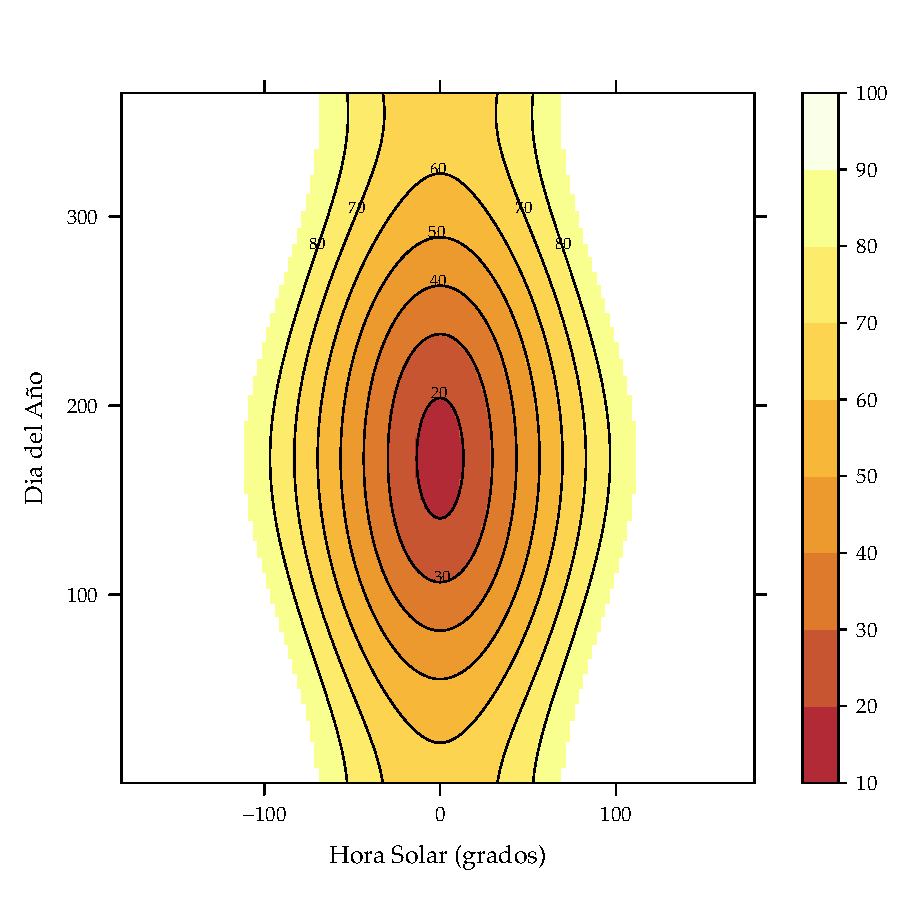
\includegraphics[scale=0.75]{../figs/BetaDoble_40N}

}

\subfloat[Orientación ($\degree$)]{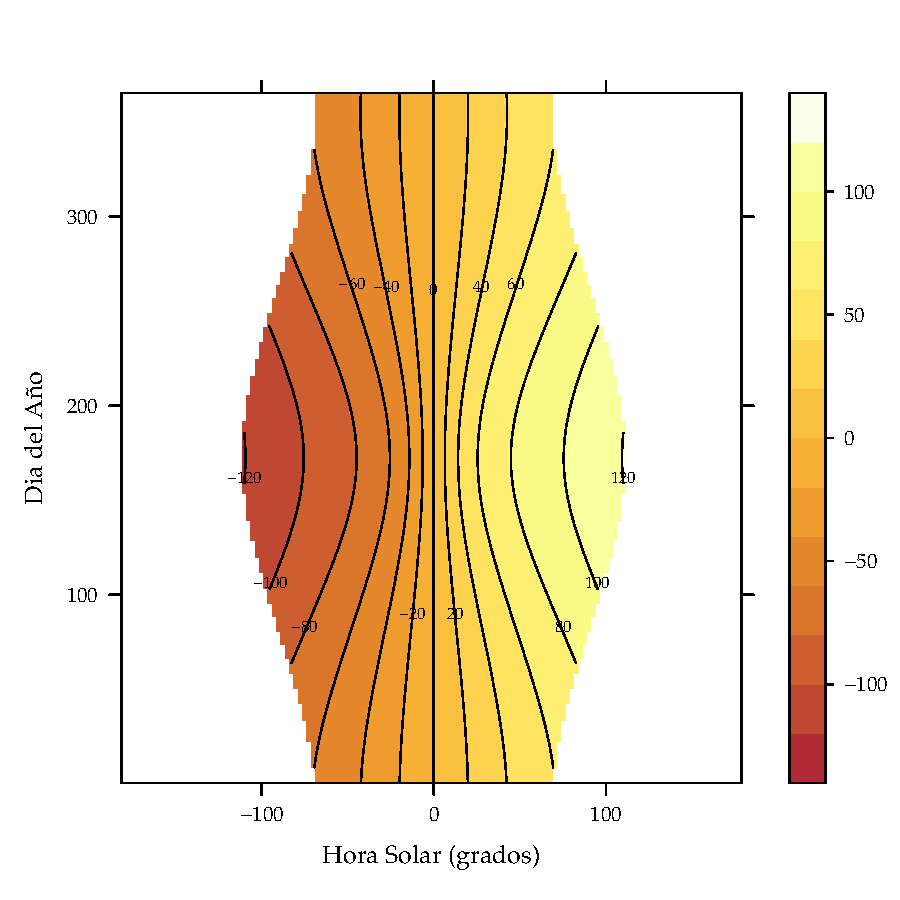
\includegraphics[scale=0.75]{../figs/AlfaDoble_40N}

}

\caption{Inclinación y orientación de un seguidor de doble eje a lo largo del
día y año para un sitio con latitud $40\degree\mathrm{N}$.\label{fig:AngulosDobleEje}}

\end{figure}


Un seguidor de eje acimutal es una versión reducida de un seguidor
de doble eje en el que la inclinación se mantiene constante a lo largo
de todo el movimiento:

\begin{align}
\beta & =cte.\\
\alpha & =\psi_{s}\\
\cos(\theta_{s}) & =\cos\left(\beta-\theta_{z}\right)\end{align}


Como puede observarse en la figura \ref{fig:cosThetaAlfa}, el ángulo
de incidencia en este seguidor toma valores no nulos en su evolución
diaria y anual. Sin embargo, es evidente la mejora respecto al seguidor
de eje horizontal y los sistemas estáticos. 

%
\begin{figure}
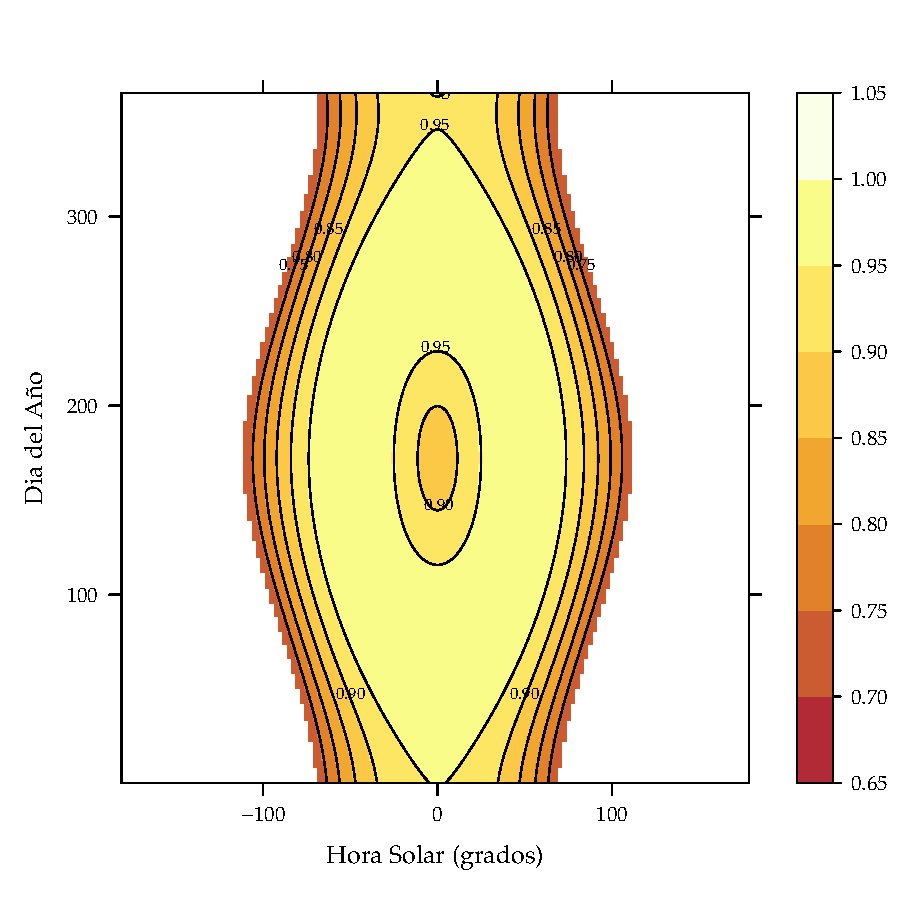
\includegraphics[scale=0.75]{../figs/cosThetaAzimutal_40N}

\caption{Coseno del ángulo de incidencia de un seguidor acimutal a lo largo
del día y año para un sitio con latitud $40\degree\mathrm{N}$.\label{fig:cosThetaAlfa}}

\end{figure}

%%% Local Variables:
%%% mode: LaTex
%%% TeX-master: "ESF.tex"
%%% End: 